\documentclass[a4paper]{article}

% Packages
\usepackage{listings}
\usepackage{color}
\usepackage[utf8]{inputenc}
\usepackage{listingsutf8}
\usepackage{graphicx}
\usepackage{epstopdf}
\usepackage{fancyhdr}
\usepackage[T1]{fontenc}
%\usepackage[top=2cm, bottom=2cm, left=3.5cm, right=2cm]{geometry} % Les marges.
\usepackage[top=2cm, bottom=2cm, left=2cm, right=2cm]{geometry} % Les marges.

\definecolor{mygreen}{rgb}{0,0.6,0}
\definecolor{mygray}{rgb}{0.5,0.5,0.5}
\definecolor{mymauve}{rgb}{0.58,0,0.82}
\definecolor{bggray}{rgb}{0.95, 0.95, 0.95}
\lstset{inputencoding=utf8/latin1}
\lstset{ %
    backgroundcolor=\color{bggray},   % choose the background color; you must add \usepackage{color} or \usepackage{xcolor}
    basicstyle=\footnotesize,        % the size of the fonts that are used for the code
    breakatwhitespace=false,         % sets if automatic breaks should only happen at whitespace
    breaklines=true,                 % sets automatic line breaking
    captionpos=b,                    % sets the caption-position to bottom
    commentstyle=\color{mygreen},    % comment style
    deletekeywords={...},            % if you want to delete keywords from the given language
    escapeinside={\%*}{*)},          % if you want to add LaTeX within your code
    extendedchars=true,              % lets you use non-ASCII characters; for 8-bits encodings only, does not work with UTF-8
    frame=single,                    % adds a frame around the code
    frameround=tttt                  % tttt for having the corner round.
    keepspaces=true,                 % keeps spaces in text, useful for keeping indentation of code (possibly needs columns=flexible)
    keywordstyle=\color{blue},       % keyword style
    language=Matlab,                 % the language of the code
    morekeywords={*,...},            % if you want to add more keywords to the set
    numbers=left,                    % where to put the line-numbers; possible values are (none, left, right)
    numbersep=5pt,                   % how far the line-numbers are from the code
    numberstyle=\tiny\color{mygray}, % the style that is used for the line-numbers
    rulecolor=\color{black},         % if not set, the frame-color may be changed on line-breaks within not-black text (e.g. comments (green here))
    showspaces=false,                % show spaces everywhere adding particular underscores; it overrides 'showstringspaces'
    showstringspaces=false,          % underline spaces within strings only
    showtabs=false,                  % show tabs within strings adding particular underscores
    stepnumber=1,                    % the step between two line-numbers. If it's 1, each line will be numbered
    stringstyle=\color{mymauve},     % string literal style
    tabsize=2,                       % sets default tabsize to 2 spaces
    title=\lstname                   % show the filename of files included with \lstinputlisting; also try caption instead of title
}

% Header
\pagestyle{fancy}
\fancyhead[L]{Axel Fahy \& Jessy Marin \& Rudolf Höhn}
\fancyhead[R]{\today}

\title{TP FFT Parallèle et application au filtrage de fréquences\\Analyse de performance}
\author{Axel Fahy \& Jessy Marin \& Rudolf Höhn}
\date{\today}

\begin{document}
\maketitle

\section{FFT Théorie}

\subsection{Complexité}
La complexité est établie en observant le nombre d'étapes que l'algorithme effectue ainsi que les différentes opérations par étape. L'algorithme FFT s'effectue en $log_2(n)$ étapes
et $n$ opérations (proportionnel donc au nombre d'éléments).\\\\
Le temps \textbf{séquentiel} se définit comme ceci :
\begin{center}
$ T_{seq} = \alpha \cdot n \cdot log_2(n) $
\end{center}
Le temps \textbf{parallèle} lui est un peu plus complexe à trouver. Le nombres d'étapes d'exécution est :
\begin{itemize}
\item \textbf{Partie sans communication} : $ T_{no\_comm} = log_2(\frac{n}{p})$ étapes
\item \textbf{Partie avec communication} : $ T_{with\_comm} = log_2(p) $ étapes
\end{itemize}
Donc, en total, il prend $log_2(n)$ étapes.\\\\
Pour calculer maintenant $T_{par}$, il faut décomposer le problème.
\begin{enumerate}
\item $T_{calculs} = \alpha \cdot \frac{n}{p} \cdot log_2(p) $
\item $T_{communicatoin} = (\gamma + \beta \cdot \frac{n}{p}) \cdot log_2(p)$
\end{enumerate}
Donc :
\begin{center}
$T_{par} = T_{calculs} + T_{communicatoin} = \alpha \cdot \frac{n}{p} \cdot log_2(n) + (\gamma + \beta \cdot \frac{n}{p}) \cdot log_2(p)$
\end{center}

\subsection{Speedup}
Le speedup théorique est : $S = \frac{T_{seq}}{T_{par}}$. Dans notre cas, le speedup est :
\begin{center}
$S = \frac{\alpha \cdot n \cdot log_2(n)}{\alpha \cdot \frac{n}{p} \cdot log_2(n) + (\gamma + \beta \cdot \frac{n}{p}) \cdot log_2(p)} = \frac{p}{1 + \frac{1}{\alpha} \cdot ( \gamma \cdot \frac{p}{n} + \beta) \cdot \frac{log_2(p)}{log_2(n)}}$
\end{center}

\subsection{Efficacité}
\begin{center}
$E(p) = \frac{S(p)}{p} = \frac{\frac{p}{1 + \frac{1}{\alpha} \cdot ( \gamma \cdot \frac{p}{n} + \beta) \cdot \frac{log_2(p)}{log_2(n)}}}{p} = \frac{1}{1 + \frac{1}{\alpha} \cdot ( \gamma \cdot \frac{p}{n} + \beta) \cdot \frac{log_2(p)}{log_2(n)}}$
\end{center}

\subsection{Isoefficacité}
Pour atteindre une efficacité constante, il faut que n et p soient une constante. Donc, $n = c \cdot p $ avec $c \ge 1$ une constante.
FFT parallèle sur une hypercube présente une bonne scalabilité.

\newpage

\section{FFT filtre sur image}

\begin{figure}[!ht]
    \center
    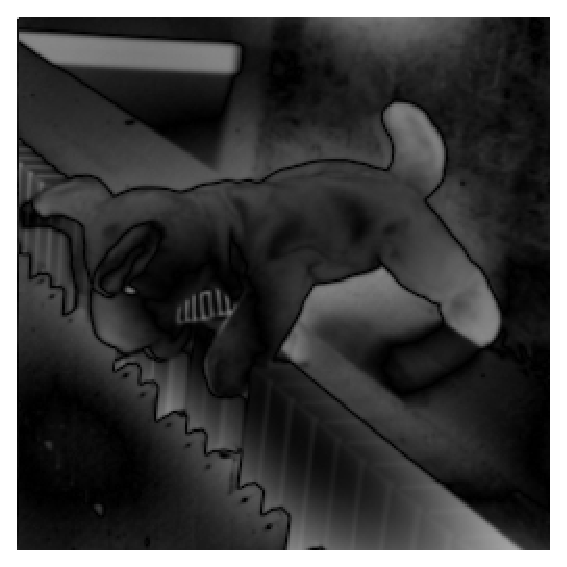
\includegraphics[width=10cm]{../images/evert_filtre_01.pgm}
    \caption{Image filtrée à 1\%}
\end{figure}

\begin{figure}[!ht]
    \center
    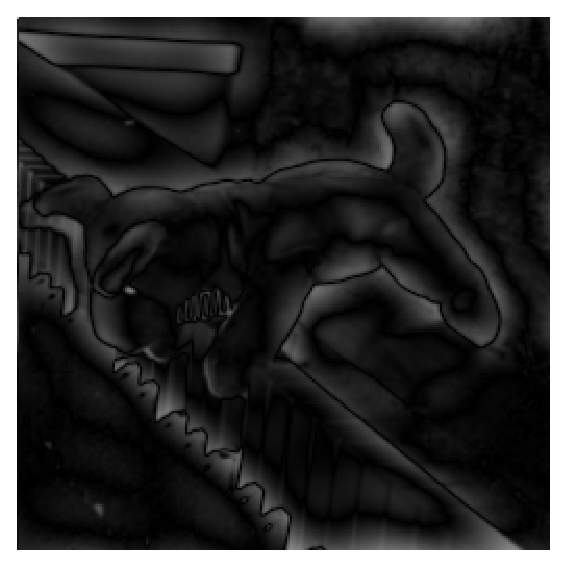
\includegraphics[width=10cm]{../images/evert_filtre_02.pgm}
    \caption{Image filtrée à 2\%}
\end{figure}

\begin{figure}[!ht]
    \center
    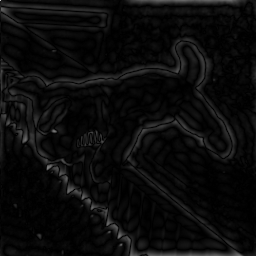
\includegraphics[width=10cm]{../images/evert_filtre_05.pgm}
    \caption{Image filtrée à 5\%}
\end{figure}

\begin{figure}[!ht]
    \center
    
\includegraphics[width=10cm]{../images/evert_filtre_10.pgm}
    \caption{Image filtrée à 10\%}
\end{figure}

\begin{figure}[!ht]
    \center
    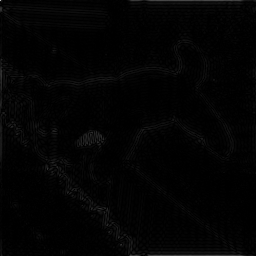
\includegraphics[width=10cm]{../images/evert_filtre_15.pgm}
    \caption{Image filtrée à 15\%}
\end{figure}

\end{document}
